% Options for packages loaded elsewhere
\PassOptionsToPackage{unicode}{hyperref}
\PassOptionsToPackage{hyphens}{url}
\PassOptionsToPackage{dvipsnames,svgnames,x11names}{xcolor}
%
\documentclass[
]{report}

\usepackage{amsmath,amssymb}
\usepackage{iftex}
\ifPDFTeX
  \usepackage[T1]{fontenc}
  \usepackage[utf8]{inputenc}
  \usepackage{textcomp} % provide euro and other symbols
\else % if luatex or xetex
  \usepackage{unicode-math}
  \defaultfontfeatures{Scale=MatchLowercase}
  \defaultfontfeatures[\rmfamily]{Ligatures=TeX,Scale=1}
\fi
\usepackage[]{libertinus}
\ifPDFTeX\else  
    % xetex/luatex font selection
\fi
% Use upquote if available, for straight quotes in verbatim environments
\IfFileExists{upquote.sty}{\usepackage{upquote}}{}
\IfFileExists{microtype.sty}{% use microtype if available
  \usepackage[]{microtype}
  \UseMicrotypeSet[protrusion]{basicmath} % disable protrusion for tt fonts
}{}
\makeatletter
\@ifundefined{KOMAClassName}{% if non-KOMA class
  \IfFileExists{parskip.sty}{%
    \usepackage{parskip}
  }{% else
    \setlength{\parindent}{0pt}
    \setlength{\parskip}{6pt plus 2pt minus 1pt}}
}{% if KOMA class
  \KOMAoptions{parskip=half}}
\makeatother
\usepackage{xcolor}
\setlength{\emergencystretch}{3em} % prevent overfull lines
\setcounter{secnumdepth}{-\maxdimen} % remove section numbering
% Make \paragraph and \subparagraph free-standing
\ifx\paragraph\undefined\else
  \let\oldparagraph\paragraph
  \renewcommand{\paragraph}[1]{\oldparagraph{#1}\mbox{}}
\fi
\ifx\subparagraph\undefined\else
  \let\oldsubparagraph\subparagraph
  \renewcommand{\subparagraph}[1]{\oldsubparagraph{#1}\mbox{}}
\fi

\usepackage{color}
\usepackage{fancyvrb}
\newcommand{\VerbBar}{|}
\newcommand{\VERB}{\Verb[commandchars=\\\{\}]}
\DefineVerbatimEnvironment{Highlighting}{Verbatim}{commandchars=\\\{\}}
% Add ',fontsize=\small' for more characters per line
\usepackage{framed}
\definecolor{shadecolor}{RGB}{241,243,245}
\newenvironment{Shaded}{\begin{snugshade}}{\end{snugshade}}
\newcommand{\AlertTok}[1]{\textcolor[rgb]{0.68,0.00,0.00}{#1}}
\newcommand{\AnnotationTok}[1]{\textcolor[rgb]{0.37,0.37,0.37}{#1}}
\newcommand{\AttributeTok}[1]{\textcolor[rgb]{0.40,0.45,0.13}{#1}}
\newcommand{\BaseNTok}[1]{\textcolor[rgb]{0.68,0.00,0.00}{#1}}
\newcommand{\BuiltInTok}[1]{\textcolor[rgb]{0.00,0.23,0.31}{#1}}
\newcommand{\CharTok}[1]{\textcolor[rgb]{0.13,0.47,0.30}{#1}}
\newcommand{\CommentTok}[1]{\textcolor[rgb]{0.37,0.37,0.37}{#1}}
\newcommand{\CommentVarTok}[1]{\textcolor[rgb]{0.37,0.37,0.37}{\textit{#1}}}
\newcommand{\ConstantTok}[1]{\textcolor[rgb]{0.56,0.35,0.01}{#1}}
\newcommand{\ControlFlowTok}[1]{\textcolor[rgb]{0.00,0.23,0.31}{#1}}
\newcommand{\DataTypeTok}[1]{\textcolor[rgb]{0.68,0.00,0.00}{#1}}
\newcommand{\DecValTok}[1]{\textcolor[rgb]{0.68,0.00,0.00}{#1}}
\newcommand{\DocumentationTok}[1]{\textcolor[rgb]{0.37,0.37,0.37}{\textit{#1}}}
\newcommand{\ErrorTok}[1]{\textcolor[rgb]{0.68,0.00,0.00}{#1}}
\newcommand{\ExtensionTok}[1]{\textcolor[rgb]{0.00,0.23,0.31}{#1}}
\newcommand{\FloatTok}[1]{\textcolor[rgb]{0.68,0.00,0.00}{#1}}
\newcommand{\FunctionTok}[1]{\textcolor[rgb]{0.28,0.35,0.67}{#1}}
\newcommand{\ImportTok}[1]{\textcolor[rgb]{0.00,0.46,0.62}{#1}}
\newcommand{\InformationTok}[1]{\textcolor[rgb]{0.37,0.37,0.37}{#1}}
\newcommand{\KeywordTok}[1]{\textcolor[rgb]{0.00,0.23,0.31}{#1}}
\newcommand{\NormalTok}[1]{\textcolor[rgb]{0.00,0.23,0.31}{#1}}
\newcommand{\OperatorTok}[1]{\textcolor[rgb]{0.37,0.37,0.37}{#1}}
\newcommand{\OtherTok}[1]{\textcolor[rgb]{0.00,0.23,0.31}{#1}}
\newcommand{\PreprocessorTok}[1]{\textcolor[rgb]{0.68,0.00,0.00}{#1}}
\newcommand{\RegionMarkerTok}[1]{\textcolor[rgb]{0.00,0.23,0.31}{#1}}
\newcommand{\SpecialCharTok}[1]{\textcolor[rgb]{0.37,0.37,0.37}{#1}}
\newcommand{\SpecialStringTok}[1]{\textcolor[rgb]{0.13,0.47,0.30}{#1}}
\newcommand{\StringTok}[1]{\textcolor[rgb]{0.13,0.47,0.30}{#1}}
\newcommand{\VariableTok}[1]{\textcolor[rgb]{0.07,0.07,0.07}{#1}}
\newcommand{\VerbatimStringTok}[1]{\textcolor[rgb]{0.13,0.47,0.30}{#1}}
\newcommand{\WarningTok}[1]{\textcolor[rgb]{0.37,0.37,0.37}{\textit{#1}}}

\providecommand{\tightlist}{%
  \setlength{\itemsep}{0pt}\setlength{\parskip}{0pt}}\usepackage{longtable,booktabs,array}
\usepackage{calc} % for calculating minipage widths
% Correct order of tables after \paragraph or \subparagraph
\usepackage{etoolbox}
\makeatletter
\patchcmd\longtable{\par}{\if@noskipsec\mbox{}\fi\par}{}{}
\makeatother
% Allow footnotes in longtable head/foot
\IfFileExists{footnotehyper.sty}{\usepackage{footnotehyper}}{\usepackage{footnote}}
\makesavenoteenv{longtable}
\usepackage{graphicx}
\makeatletter
\def\maxwidth{\ifdim\Gin@nat@width>\linewidth\linewidth\else\Gin@nat@width\fi}
\def\maxheight{\ifdim\Gin@nat@height>\textheight\textheight\else\Gin@nat@height\fi}
\makeatother
% Scale images if necessary, so that they will not overflow the page
% margins by default, and it is still possible to overwrite the defaults
% using explicit options in \includegraphics[width, height, ...]{}
\setkeys{Gin}{width=\maxwidth,height=\maxheight,keepaspectratio}
% Set default figure placement to htbp
\makeatletter
\def\fps@figure{htbp}
\makeatother

\makeatletter
\makeatother
\makeatletter
\makeatother
\makeatletter
\@ifpackageloaded{caption}{}{\usepackage{caption}}
\AtBeginDocument{%
\ifdefined\contentsname
  \renewcommand*\contentsname{Table of contents}
\else
  \newcommand\contentsname{Table of contents}
\fi
\ifdefined\listfigurename
  \renewcommand*\listfigurename{List of Figures}
\else
  \newcommand\listfigurename{List of Figures}
\fi
\ifdefined\listtablename
  \renewcommand*\listtablename{List of Tables}
\else
  \newcommand\listtablename{List of Tables}
\fi
\ifdefined\figurename
  \renewcommand*\figurename{Figure}
\else
  \newcommand\figurename{Figure}
\fi
\ifdefined\tablename
  \renewcommand*\tablename{Table}
\else
  \newcommand\tablename{Table}
\fi
}
\@ifpackageloaded{float}{}{\usepackage{float}}
\floatstyle{ruled}
\@ifundefined{c@chapter}{\newfloat{codelisting}{h}{lop}}{\newfloat{codelisting}{h}{lop}[chapter]}
\floatname{codelisting}{Listing}
\newcommand*\listoflistings{\listof{codelisting}{List of Listings}}
\makeatother
\makeatletter
\@ifpackageloaded{caption}{}{\usepackage{caption}}
\@ifpackageloaded{subcaption}{}{\usepackage{subcaption}}
\makeatother
\makeatletter
\@ifpackageloaded{tcolorbox}{}{\usepackage[skins,breakable]{tcolorbox}}
\makeatother
\makeatletter
\@ifundefined{shadecolor}{\definecolor{shadecolor}{rgb}{.97, .97, .97}}
\makeatother
\makeatletter
\makeatother
\makeatletter
\makeatother
\ifLuaTeX
  \usepackage{selnolig}  % disable illegal ligatures
\fi
\IfFileExists{bookmark.sty}{\usepackage{bookmark}}{\usepackage{hyperref}}
\IfFileExists{xurl.sty}{\usepackage{xurl}}{} % add URL line breaks if available
\urlstyle{same} % disable monospaced font for URLs
\hypersetup{
  pdftitle={Linear Models},
  pdfauthor={Abhishek Swain},
  colorlinks=true,
  linkcolor={blue},
  filecolor={Maroon},
  citecolor={Blue},
  urlcolor={Blue},
  pdfcreator={LaTeX via pandoc}}

\title{Linear Models}
\author{Abhishek Swain}
\date{2023-09-16}

\begin{document}
\maketitle
\ifdefined\Shaded\renewenvironment{Shaded}{\begin{tcolorbox}[boxrule=0pt, interior hidden, enhanced, sharp corners, borderline west={3pt}{0pt}{shadecolor}, frame hidden, breakable]}{\end{tcolorbox}}\fi

\renewcommand*\contentsname{Table of Contents}
{
\hypersetup{linkcolor=}
\setcounter{tocdepth}{2}
\tableofcontents
}
\listoffigures
\hypertarget{linear-regression}{%
\chapter{Linear Regression}\label{linear-regression}}

\begin{Shaded}
\begin{Highlighting}[]
\ImportTok{import}\NormalTok{ numpy }\ImportTok{as}\NormalTok{ np}
\ImportTok{import}\NormalTok{ matplotlib.pyplot }\ImportTok{as}\NormalTok{ plt}
\ImportTok{from}\NormalTok{ sklearn.preprocessing }\ImportTok{import}\NormalTok{ add\_dummy\_feature, PolynomialFeatures}
\ImportTok{from}\NormalTok{ sklearn.linear\_model }\ImportTok{import}\NormalTok{ LinearRegression, SGDRegressor}

\ImportTok{import}\NormalTok{ warnings}
\NormalTok{warnings.filterwarnings(}\StringTok{"ignore"}\NormalTok{)}
\end{Highlighting}
\end{Shaded}

\hypertarget{the-equations}{%
\section{The Equations}\label{the-equations}}

\hypertarget{standard-equation}{%
\subsection{Standard equation}\label{standard-equation}}

\(\hat{y} = \theta_{0} + \theta_{1}x_{1} + \theta_{2}x_{2} + \dots + \theta_{n}x_{n}\)

\begin{itemize}
\tightlist
\item
  \(\hat{y}\) is the predicted value.
\item
  n is the number of features.
\item
  \(x_{i}\) is the \(i^{th}\) feature value.
\item
  \(\theta_{j}\) is the \(j^{th}\) model parameter.
\end{itemize}

\hypertarget{vectorized-equation}{%
\subsection{Vectorized equation}\label{vectorized-equation}}

\(\hat{y} = h_{\theta}(x) = \theta \cdot x\)

\begin{itemize}
\tightlist
\item
  \(\theta\) here is the model's parameter containing
  \(\theta_{0} \dots \theta_{n}\).
\item
  \(x\) is the features containing \(x_{0} \dots x_{n}\) where \(x_{0}\)
  is always 1.
\item
  \(\theta \cdot x\) is the dot product between \(\theta\) \& x. Both
  are colum vectors.
\end{itemize}

\(\hat{y} = \theta \cdot x = \theta^{T}x = [\theta_{0} \dots \theta_{n}] \begin{bmatrix} x_{0} \\ \vdots \\ x_{n}\end{bmatrix} = \theta_{0} + \theta_{1}x_{1} + \theta_{2}x_{2} + \dots + \theta_{n}x_{n}\)

where \(x_{0} = 1\)

\hypertarget{training-the-model}{%
\section{Training the model}\label{training-the-model}}

We need a loss function to train this model. Out loss funciton is MSE
loss.

\(MSE(X, h_{\theta}) = \frac{1}{m} \sum_{i=1}^m (\theta^T x^{(i)} - y^{(i)})^2\)

Here \((i)\) is the \(i^{th}\) training example.

\hypertarget{the-normal-equation}{%
\subsection{The Normal Equation}\label{the-normal-equation}}

Without using any optimization algorithm we also have a direct formula
to get the parameters, this formula is the \emph{Normal Equation}

\(\hat{\theta} = (X^{T}X)^{-1} X^{T} y\)

\begin{itemize}
\tightlist
\item
  \(\hat{\theta}\) is the estimated parameter,
  \(\hat{\theta} \approx \theta\)
\item
  \(y\) is is the target vector containing \(y^{(1)} \dots y^{(m)}\)
\end{itemize}

\hypertarget{examples}{%
\subsubsection{Examples}\label{examples}}

\begin{Shaded}
\begin{Highlighting}[]
\CommentTok{\# Generate dummy data}

\NormalTok{np.random.seed(}\DecValTok{42}\NormalTok{)}
\NormalTok{m }\OperatorTok{=} \DecValTok{100}
\NormalTok{X }\OperatorTok{=} \DecValTok{2} \OperatorTok{*}\NormalTok{ np.random.randn(m, }\DecValTok{1}\NormalTok{)}
\NormalTok{y }\OperatorTok{=} \DecValTok{3} \OperatorTok{*}\NormalTok{ X }\OperatorTok{+}\NormalTok{ np.random.randn(m, }\DecValTok{1}\NormalTok{)}

\CommentTok{\# Add bias term to X}
\NormalTok{X\_b }\OperatorTok{=}\NormalTok{ add\_dummy\_feature(X)}
\end{Highlighting}
\end{Shaded}

\begin{Shaded}
\begin{Highlighting}[]
\NormalTok{X\_b.shape, y.shape}
\end{Highlighting}
\end{Shaded}

\begin{verbatim}
((100, 2), (100, 1))
\end{verbatim}

\begin{Shaded}
\begin{Highlighting}[]
\NormalTok{best\_theta }\OperatorTok{=}\NormalTok{ np.linalg.inv(X\_b.T }\OperatorTok{@}\NormalTok{ X\_b) }\OperatorTok{@}\NormalTok{ X\_b.T }\OperatorTok{@}\NormalTok{ y }\CommentTok{\# Using the normal eqaution}
\end{Highlighting}
\end{Shaded}

\begin{Shaded}
\begin{Highlighting}[]
\NormalTok{best\_theta}
\end{Highlighting}
\end{Shaded}

\begin{verbatim}
array([[0.00742783],
       [2.92837142]])
\end{verbatim}

The equation is \(y = 3x + \text{Gaussian Noise}\), and you can see that
the estimated \(\theta_{1}\) is \(2.9 \approx 3\) and \(\theta_{0} = 0\)

\begin{Shaded}
\begin{Highlighting}[]
\CommentTok{\# Make some predictions}

\NormalTok{X\_new }\OperatorTok{=}\NormalTok{ np.array([[}\DecValTok{0}\NormalTok{], [}\DecValTok{2}\NormalTok{]])}
\NormalTok{X\_new }\OperatorTok{=}\NormalTok{ add\_dummy\_feature(X\_new)}
\end{Highlighting}
\end{Shaded}

\begin{Shaded}
\begin{Highlighting}[]
\NormalTok{y\_pred }\OperatorTok{=}\NormalTok{ X\_new }\OperatorTok{@}\NormalTok{ best\_theta}
\end{Highlighting}
\end{Shaded}

\begin{Shaded}
\begin{Highlighting}[]
\NormalTok{y\_pred}
\end{Highlighting}
\end{Shaded}

\begin{verbatim}
array([[0.00742783],
       [5.86417067]])
\end{verbatim}

\hypertarget{linear-regression-with-scikit-learn}{%
\subsection{\texorpdfstring{Linear Regression with
\texttt{scikit-learn}}{Linear Regression with scikit-learn}}\label{linear-regression-with-scikit-learn}}

\begin{Shaded}
\begin{Highlighting}[]
\NormalTok{lr }\OperatorTok{=}\NormalTok{ LinearRegression()}
\NormalTok{lr.fit(X\_b, y)}
\end{Highlighting}
\end{Shaded}

\begin{verbatim}
LinearRegression()
\end{verbatim}

\begin{Shaded}
\begin{Highlighting}[]
\NormalTok{lr.coef\_}
\end{Highlighting}
\end{Shaded}

\begin{verbatim}
array([[0.        , 2.92837142]])
\end{verbatim}

The \texttt{LinearRegression} in \texttt{sklearn} computes \(X^{+}y\)
where \(X_{+}\) is the pseudoinverse (Moore - Penrose pseudoinverse). We
can compute it directly using \texttt{np.linalg.pinv}

\begin{Shaded}
\begin{Highlighting}[]
\NormalTok{np.linalg.pinv(X\_b) }\OperatorTok{@}\NormalTok{ y}
\end{Highlighting}
\end{Shaded}

\begin{verbatim}
array([[0.00742783],
       [2.92837142]])
\end{verbatim}

\hypertarget{computational-complexity}{%
\subsection{Computational Complexity}\label{computational-complexity}}

\begin{itemize}
\tightlist
\item
  Computing the inverse of \(X^{T}X\) which is (n + 1) x (n + 1) matrix
  upto \(O(n^{3})\). The scikit-learn Linear Regression is almost
  \(O(n^{2})\)
\item
  However, once computed, time to make predictions is very fast. It
  scales \(O(n)\) with the number of predictions to be made
\end{itemize}

\hypertarget{gradient-descent}{%
\subsection{Gradient Descent}\label{gradient-descent}}

\begin{itemize}
\tightlist
\item
  This is an iterative method to find the parameters of the model
\item
  We compute the gradient of the loss function at a particular point and
  move in the direction of the -ve gradient (the steepest descent)
\end{itemize}

Ex: You want to go down hill from a the top but it is very foggy, you
use your feet to find the next steepest descent point

We are basically searching in the model's parameter space, so more the
parameters, the harder the search becomes.

Factors affecting search: - Learning rate determines how big of a step
we are taking, too big and we may overshoot - Shape of the function, if
the loss function is complex (has lots of highs and toughs) there are
chances our GD may get stuck in a \emph{Local Minima} \& not the
\emph{Global Minima}

Fortunately, MSE is a convex function all we do is go down the slope to
the bottom of the bowl

\hypertarget{batch-gradient-descent}{%
\subsubsection{Batch Gradient Descent}\label{batch-gradient-descent}}

To implement GD we need to compute the partial derivative of the Loss
function with each parameter of the model

\(MSE(\theta) = \frac{1}{m} \sum_{i=1}^m (\theta^T x^{(i)} - y^{(i)})^2\)

\(\frac{\partial MSE(\theta)}{\partial \theta_{j}} = \frac{2}{m} \sum_{i=1}^m (\theta^T x^{(i)} - y^{(i)}) x_{j}\)

Rather than computing them one-by-one, we vectorize the whole stuff,

\(\nabla_{\theta}MSE(\theta) = \begin{bmatrix} \frac{\partial MSE(\theta)}{\partial \theta_{0}} \\ \frac{\partial MSE(\theta)}{\partial \theta_{1}} \\ \vdots \\ \frac{\partial MSE(\theta)}{\partial \theta_{n}} \end{bmatrix} = \frac{2}{m} X^{T} (X\theta - y)\)

The gradient descent step:

\(\theta = \theta - \eta\nabla_{\theta}MSE(\theta)\)

\begin{Shaded}
\begin{Highlighting}[]
\CommentTok{\# Quick implementation}

\NormalTok{lr }\OperatorTok{=} \FloatTok{0.1}
\NormalTok{n\_epochs }\OperatorTok{=} \DecValTok{1000}

\NormalTok{m }\OperatorTok{=} \BuiltInTok{len}\NormalTok{(X\_b)}

\NormalTok{theta }\OperatorTok{=}\NormalTok{ np.random.randn(}\DecValTok{2}\NormalTok{, }\DecValTok{1}\NormalTok{) }\CommentTok{\# Sample theta from Gaussian distribution}

\ControlFlowTok{for}\NormalTok{ \_ }\KeywordTok{in} \BuiltInTok{range}\NormalTok{(n\_epochs):}
\NormalTok{    grad }\OperatorTok{=}\NormalTok{ (}\DecValTok{2}\OperatorTok{/}\NormalTok{m) }\OperatorTok{*}\NormalTok{ X\_b.T }\OperatorTok{@}\NormalTok{ (X\_b }\OperatorTok{@}\NormalTok{ theta }\OperatorTok{{-}}\NormalTok{  y)}
\NormalTok{    theta }\OperatorTok{=}\NormalTok{ theta }\OperatorTok{{-}}\NormalTok{ lr }\OperatorTok{*}\NormalTok{ grad}
\end{Highlighting}
\end{Shaded}

\begin{Shaded}
\begin{Highlighting}[]
\NormalTok{theta}
\end{Highlighting}
\end{Shaded}

\begin{verbatim}
array([[0.00742783],
       [2.92837142]])
\end{verbatim}

\begin{Shaded}
\begin{Highlighting}[]
\NormalTok{best\_theta}
\end{Highlighting}
\end{Shaded}

\begin{verbatim}
array([[0.00742783],
       [2.92837142]])
\end{verbatim}

As we can see that the value we got from the normal equation and through
GD is the same!

\hypertarget{stochastic-gradient-descent}{%
\subsubsection{Stochastic Gradient
Descent}\label{stochastic-gradient-descent}}

\begin{itemize}
\tightlist
\item
  The issue with batch gradient descent is that it goes through the
  whole traininig set at once, making it very slow when the training set
  is huge. To solve this a better approach is SGD. It picks a random
  instance from the traning set and calculates the gradient based on
  that instance.
\item
  This causes the loss value to bounce up and down. So unlile BGD we
  will not see a gradual decrease but only seeing a decrease in loss on
  average.
\item
  This causes the loss to never settle even after reaching a minimum
  that also helps it get out of a local minima better than BGD.
\item
  To solve this we can use something called ``simulated annealing'', in
  which we keep decreasing the learning rate gradually (learning
  schedule).
\end{itemize}

\begin{Shaded}
\begin{Highlighting}[]
\CommentTok{\# Implementation}

\NormalTok{n\_epochs }\OperatorTok{=} \DecValTok{50}

\NormalTok{t0, t1 }\OperatorTok{=} \DecValTok{5}\NormalTok{, }\DecValTok{50}

\NormalTok{m }\OperatorTok{=}  \BuiltInTok{len}\NormalTok{(X\_b)}

\NormalTok{theta }\OperatorTok{=}\NormalTok{ np.random.randn(}\DecValTok{2}\NormalTok{, }\DecValTok{1}\NormalTok{)}

\KeywordTok{def}\NormalTok{ learning\_schedule(t):}
    \ControlFlowTok{return}\NormalTok{ t0 }\OperatorTok{/}\NormalTok{ (t }\OperatorTok{+}\NormalTok{ t1)}

\ControlFlowTok{for}\NormalTok{ epoch }\KeywordTok{in} \BuiltInTok{range}\NormalTok{(n\_epochs):}
    \ControlFlowTok{for}\NormalTok{ i }\KeywordTok{in} \BuiltInTok{range}\NormalTok{(m):}
\NormalTok{        idx }\OperatorTok{=}\NormalTok{ np.random.randint(m)}
\NormalTok{        Xi }\OperatorTok{=}\NormalTok{ X\_b[idx:]}
\NormalTok{        yi }\OperatorTok{=}\NormalTok{ y[idx:]}
        
\NormalTok{        grad }\OperatorTok{=} \DecValTok{2} \OperatorTok{*}\NormalTok{ Xi.T }\OperatorTok{@}\NormalTok{ (Xi }\OperatorTok{@}\NormalTok{ theta }\OperatorTok{{-}}\NormalTok{ yi) }\CommentTok{\# Do not divide by m, as it\textquotesingle{}s a single instance}
\NormalTok{        theta }\OperatorTok{=}\NormalTok{ theta }\OperatorTok{{-}}\NormalTok{ learning\_schedule(epoch }\OperatorTok{*}\NormalTok{ m }\OperatorTok{+}\NormalTok{ i) }\OperatorTok{*}\NormalTok{ grad    }
\end{Highlighting}
\end{Shaded}

\begin{Shaded}
\begin{Highlighting}[]
\NormalTok{theta}
\end{Highlighting}
\end{Shaded}

\begin{verbatim}
array([[0.01630277],
       [2.92664477]])
\end{verbatim}

We arrive at almost the same values but with just 50 epochs

\begin{quote}
All data need to be Identically and Independently distributed (IID) for
SGD to work correctly, if the data is sorted by label then it will start
optimizing for only one label.
\end{quote}

\hypertarget{sgd-with-scikit-learn}{%
\subsubsection{\texorpdfstring{SGD with
\texttt{scikit-learn}}{SGD with scikit-learn}}\label{sgd-with-scikit-learn}}

\begin{Shaded}
\begin{Highlighting}[]
\NormalTok{sgd }\OperatorTok{=}\NormalTok{ SGDRegressor(}
\NormalTok{    max\_iter}\OperatorTok{=}\DecValTok{1000}\NormalTok{, }
\NormalTok{    tol}\OperatorTok{=}\FloatTok{1e{-}5}\NormalTok{, }
\NormalTok{    eta0}\OperatorTok{=}\FloatTok{0.01}\NormalTok{, }
\NormalTok{    n\_iter\_no\_change}\OperatorTok{=}\DecValTok{100}\NormalTok{, }
\NormalTok{    random\_state}\OperatorTok{=}\DecValTok{42}
\NormalTok{)}
\NormalTok{sgd.fit(X\_b, y.ravel())}
\end{Highlighting}
\end{Shaded}

\begin{verbatim}
SGDRegressor(n_iter_no_change=100, random_state=42, tol=1e-05)
\end{verbatim}

\begin{Shaded}
\begin{Highlighting}[]
\NormalTok{sgd.coef\_}
\end{Highlighting}
\end{Shaded}

\begin{verbatim}
array([0.00404065, 2.92966112])
\end{verbatim}

\hypertarget{mini-batch-gradient-descent}{%
\subsubsection{Mini batch Gradient
Descent}\label{mini-batch-gradient-descent}}

\begin{Shaded}
\begin{Highlighting}[]
\NormalTok{batches }\OperatorTok{=}\NormalTok{ [(X\_b[i:i}\OperatorTok{+}\DecValTok{10}\NormalTok{], y[i:i}\OperatorTok{+}\DecValTok{10}\NormalTok{]) }\ControlFlowTok{for}\NormalTok{ i }\KeywordTok{in} \BuiltInTok{range}\NormalTok{(}\DecValTok{0}\NormalTok{, }\BuiltInTok{len}\NormalTok{(X\_b), }\DecValTok{10}\NormalTok{)]}
\end{Highlighting}
\end{Shaded}

\begin{Shaded}
\begin{Highlighting}[]
\NormalTok{n\_epochs }\OperatorTok{=} \DecValTok{30}
\NormalTok{theta }\OperatorTok{=}\NormalTok{ np.random.randn(}\DecValTok{2}\NormalTok{, }\DecValTok{1}\NormalTok{)}
\NormalTok{lr }\OperatorTok{=} \FloatTok{0.01}

\ControlFlowTok{for}\NormalTok{ epoch }\KeywordTok{in} \BuiltInTok{range}\NormalTok{(n\_epochs):}
    \ControlFlowTok{for}\NormalTok{ xi, yi }\KeywordTok{in}\NormalTok{ batches:}
\NormalTok{        m }\OperatorTok{=} \BuiltInTok{len}\NormalTok{(xi)}
\NormalTok{        grad }\OperatorTok{=}\NormalTok{ (}\DecValTok{2}\OperatorTok{/}\NormalTok{m) }\OperatorTok{*}\NormalTok{ xi.T }\OperatorTok{@}\NormalTok{ (xi }\OperatorTok{@}\NormalTok{ theta }\OperatorTok{{-}}\NormalTok{ yi)}
\NormalTok{        theta }\OperatorTok{=}\NormalTok{ theta }\OperatorTok{{-}}\NormalTok{ lr }\OperatorTok{*}\NormalTok{ grad   }
\end{Highlighting}
\end{Shaded}

\begin{Shaded}
\begin{Highlighting}[]
\NormalTok{theta}
\end{Highlighting}
\end{Shaded}

\begin{verbatim}
array([[0.00396903],
       [2.92040931]])
\end{verbatim}

\hypertarget{polynomial-regression}{%
\chapter{Polynomial Regression}\label{polynomial-regression}}

\begin{Shaded}
\begin{Highlighting}[]
\NormalTok{np.random.seed(}\DecValTok{42}\NormalTok{)}
\NormalTok{m }\OperatorTok{=} \DecValTok{200}
\NormalTok{X }\OperatorTok{=} \DecValTok{6} \OperatorTok{*}\NormalTok{ np.random.randn(m, }\DecValTok{1}\NormalTok{)}
\NormalTok{y }\OperatorTok{=} \DecValTok{3} \OperatorTok{*}\NormalTok{ X }\OperatorTok{**} \DecValTok{2} \OperatorTok{+}\NormalTok{ X }\OperatorTok{+} \DecValTok{2} \OperatorTok{+}\NormalTok{ np.random.randn(m, }\DecValTok{1}\NormalTok{)}
\end{Highlighting}
\end{Shaded}

\begin{Shaded}
\begin{Highlighting}[]
\NormalTok{plt.plot(X, y, }\StringTok{"b."}\NormalTok{)}
\NormalTok{plt.show()}
\end{Highlighting}
\end{Shaded}

\begin{figure}[H]

{\centering 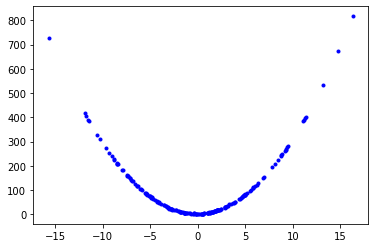
\includegraphics{LinearModels_files/figure-pdf/random-polynomial-data-output-1.png}

}

\caption{Random Polynomial data}

\end{figure}

\begin{Shaded}
\begin{Highlighting}[]
\NormalTok{lr }\OperatorTok{=}\NormalTok{ LinearRegression()}
\NormalTok{lr.fit(X, y)}
\end{Highlighting}
\end{Shaded}

\begin{verbatim}
LinearRegression()
\end{verbatim}

\begin{Shaded}
\begin{Highlighting}[]
\NormalTok{lr.coef\_, lr.intercept\_}
\end{Highlighting}
\end{Shaded}

\begin{verbatim}
(array([[1.76348997]]), array([95.59508332]))
\end{verbatim}

Simple LR doesn't do well, that is expected. We need to create some
polynomial features

\begin{Shaded}
\begin{Highlighting}[]
\NormalTok{X\_poly }\OperatorTok{=}\NormalTok{ PolynomialFeatures(include\_bias}\OperatorTok{=}\VariableTok{False}\NormalTok{).fit\_transform(X)}
\end{Highlighting}
\end{Shaded}

\begin{Shaded}
\begin{Highlighting}[]
\NormalTok{lr.fit(X\_poly, y)}
\end{Highlighting}
\end{Shaded}

\begin{verbatim}
LinearRegression()
\end{verbatim}

\begin{Shaded}
\begin{Highlighting}[]
\NormalTok{lr.coef\_, lr.intercept\_}
\end{Highlighting}
\end{Shaded}

\begin{verbatim}
(array([[1.01748959, 2.99727606]]), array([2.17488155]))
\end{verbatim}

This does so much better, our equation
\(y = 3X^{2} + X + 2 + \text{Gaussian Noise}\), the predicted equation
is \(y = 2.99X^{2} + 1.017 X + 2.17\)

\hypertarget{biasvariance-tradeoff}{%
\chapter{Bias/Variance Tradeoff}\label{biasvariance-tradeoff}}

Model's generalization error is a sum of 3 different error:

\begin{enumerate}
\def\labelenumi{\arabic{enumi}.}
\tightlist
\item
  \textbf{Bias}:
\end{enumerate}

\begin{itemize}
\tightlist
\item
  Arising due to wrong assumptions like thinking data is linear when it
  is quadratic.
\item
  \emph{High Bias} model mostly \emph{Underfits}.
\end{itemize}

\begin{enumerate}
\def\labelenumi{\arabic{enumi}.}
\setcounter{enumi}{1}
\tightlist
\item
  \textbf{Variance}:
\end{enumerate}

\begin{itemize}
\tightlist
\item
  Arising due to model's excessive sensitivity to small variations in
  the data.
\item
  Model with high degrees of freedom likely has high variance.
\item
  \emph{High Variance} model mostly \emph{Overfits}.
\end{itemize}

\begin{enumerate}
\def\labelenumi{\arabic{enumi}.}
\setcounter{enumi}{2}
\tightlist
\item
  \textbf{Irreducible Error}
\end{enumerate}

\begin{itemize}
\tightlist
\item
  Arising due to noise in data.
\item
  Only way to solve is to clean the data.
\end{itemize}



\end{document}
